% !TEX root = sycl-1.2.1.tex

\chapter{SYCL Architecture}

This chapter builds on the structure of the OpenCL specification's architecture
chapter to explain how SYCL overlays the OpenCL specification and inherits its
capabilities and restrictions as well as the additional features it provides on
top of OpenCL 1.2.

\section{Overview}

SYCL is an open industry standard for programming a heterogeneous system. The
design of SYCL allows standard C++ source code to be written such that it can
run on either an OpenCL device or on the \gls{host}.

The terminology used for SYCL inherits that of OpenCL with some
SYCL-specific additions. A function object that can execute on either
an OpenCL \gls{device} or a \gls{host} \gls{device} is called a
\gls{sycl-kernel-function}.

To ensure maximum backward-compatibility, a software developer can produce
a program that mixes standard OpenCL C kernels and OpenCL API code with
SYCL code and expect fully compatible interoperation.

The target users of SYCL are C++ programmers who want all the performance and
portability features of OpenCL, but with the flexibility to use higher-level C++
abstractions across the host/device code boundary. Developers can use most of
the abstraction features of C++, such as templates, classes and operator
overloading. However, some C++ language features are not permitted inside
kernels, due to the limitations imposed by the capabilities of the underlying
OpenCL standard. These features include virtual functions, virtual inheritance,
throwing/catching exceptions, and run-time type-information. These features are
available outside kernels as normal. Within these constraints, developers can
use abstractions defined by SYCL, or they can develop their own on top. These
capabilities make SYCL ideal for library developers, middleware providers and
applications developers who want to separate low-level highly-tuned algorithms
or data structures that work on heterogeneous systems from higher-level software
development. OpenCL developers can produce templated algorithms that are easily
usable by developers in other fields.

\newpage
\section{Anatomy of a SYCL application}

Below is an example of a typical \gls{sycl-application} which schedules a job to run
in parallel on any OpenCL device.

\lstset{
         numbers=left,
         stepnumber=1,
         numberfirstline=false
 }
\lstinputlisting{code/anatomy.cpp}

At line 1, we ``\codeinline{#include}'' the SYCL header files, which
provide all of the SYCL features that will be used.

A SYCL application runs on a SYCL Platform (see Section~\ref{sec:platformmodel}).
The application is structured in three scopes which specify the different sections;
\gls{application-scope}, \gls{command-group-scope} and \gls{kernel-scope}.
The \gls{kernel-scope} specifies a single kernel function that will
be, or has been, compiled by a \gls{device-compiler} and executed on a
\gls{device}. In this example \gls{kernel-scope} is defined by lines
25 to 27.  The \gls{command-group-scope} specifies a unit of work which will
comprise of a \gls{sycl-kernel-function} and \glspl{accessor}.  In this
example \gls{command-group-scope} is defined by lines 20 to 28.  The
\gls{application-scope} specifies all other code outside of a
\gls{command-group-scope}.  
These three scopes are used to control the
application flow and the construction and lifetimes of the various objects used
within SYCL, as explained in Section~\ref{sec:managing-object-lifetimes}.

A \gls{sycl-kernel-function} is the scoped block of code that will be
compiled using a device compiler.  This code may be defined by the
body of a lambda function, by the \codeinline{operator()} function of
a function object or by the binary \codeinline{cl_kernel} entity
generated from an OpenCL C string.  Each instance of the
\gls{sycl-kernel-function} will be executed as a single, though not
necessarily entirely independent, flow of execution and has to adhere
to restrictions on what operations may be allowed to enable device
compilers to safely compile it to a range of underlying devices.

The \codeinline{parallel_for} function is templated with a class, in this case
called \codeinline{class simple_test}. This class is used only as a name to
enable the kernel (compiled with a device compiler) and the host code (possibly
compiled with a different host compiler) to be linked. This is required
because C++ lambda functions have no name that a linker could use to link the
kernel to the host code.

The \codeinline{parallel_for} method creates an instance of a kernel object.
The kernel object is the entity that will be enqueued within a
command group.  In the case of \codeinline{parallel_for} the
\gls{sycl-kernel-function} will be executed over the given range from 0 to 1023.
The different methods to
execute kernels can be found in Section~\ref{subsec:invokingkernels}.

A \gls{sycl-kernel-function} can only be defined within a
\gls{command-group-scope}, and a \gls{command-group-scope} may include
only a single \gls{sycl-kernel-function}. Command group scope is the
syntactic scope wrapped by the construction of a
\gls{command-group-function-object} as seen on line 20. The
\gls{command-group-function-object} takes as a parameter a command
group \codeinline{handler} which is a runtime constructed object.

All the requirements for a kernel to execute are defined in this
\gls{command-group-scope}, as described in
Section~\ref{sec:executionmodel}.  In this case the constructor used
for \codeinline{myQueue} on line 14 is the default constructor, which
allows the queue to select the best underlying device to execute on,
leaving the decision up to the runtime.

In SYCL, data that is required within a \gls{sycl-kernel-function} must
be contained within a \gls{buffer} or \gls{image}, as described in
Section~\ref{sec:memory.model}. We
construct a buffer on line 17. Access to the \gls{buffer} is controlled via
an \gls{accessor} which is constructed on line 22 through the
\codeinline{get_access} method of the buffer. The \gls{buffer} is used to
keep track of access to the data and the \gls{accessor} is used to request
access to the data on a queue, as well as to track the dependencies between
\gls{sycl-kernel-function}. In this example the \gls{accessor} is used to
write to the data buffer on line 26. All \glspl{buffer} must be constructed
in the application-scope, whereas all \glspl{accessor}
must be constructed in the \gls{command-group-scope}.


\section{The SYCL Platform Model}
\label{sec:platformmodel}

The SYCL platform model is based on the OpenCL platform model, but there
are a few additional abstractions available to programmers.

The model consists of a host connected to one or more OpenCL devices.  An OpenCL
device is divided into one or more compute units (CUs) which are each divided
into one or more processing elements (PEs).  Computations on a device occur
within the processing elements.  A SYCL application runs on a host according to
the standard C++ CPU execution model.  The SYCL application submits
\glspl{command-group-function-object} to \glspl{queue}, which execute either on
OpenCL devices or on the \gls{host-device}.

When a SYCL implementation executes kernels on an OpenCL
device, it achieves this by enqueuing OpenCL \textbf{commands} to
execute computations on the processing elements within a device.  The
processing elements within an OpenCL compute unit may execute a single
stream of instructions as ALUs within a SIMD unit (which execute in
lockstep with a single stream of instructions), as independent SPMD
units (where each PE maintains its own program counter) or as some
combination of the two.

When a SYCL implementation executes kernels on the host device,
it is free to use whatever parallel execution facilities are available on the
host, as long as it executes within the semantics of the kernel execution model
defined by OpenCL.

\subsection{Platform Mixed Version Support}

OpenCL is designed to support devices with different capabilities under a
single platform.  This includes devices which conform to different
versions of the OpenCL specification and devices which support different
extensions to the OpenCL specification.  There are three important sets of
capabilities to consider for a SYCL device: the platform version, the
version of a device and the extensions supported.

The SYCL system presents the user with a set of devices, grouped into some
number of platforms.
The device version is an indication of the device's
capabilities, as represented by the device information returned by the
\codeinline{cl::sycl::device::get_info()} method.  Examples of attributes
associated with the device version are resource limits and information
about functionality beyond the core OpenCL specification's requirements.
The version returned corresponds to the highest version of the OpenCL
specification for which the device is conformant, but is not higher than
the version of the device's platform which bounds the overall capabilities
of the runtime operating the device.

In OpenCL, a device has a \keyword{language version}. In SYCL, the source
language is compiled offline, so the language version is not available at
runtime.  Instead, the SYCL language version is available as a
compile-time macro: \codeinline{CL_SYCL_LANGUAGE_VERSION}.


\section{SYCL Execution Model}

The execution of a SYCL program occurs in two parts:
\glspl{sycl-kernel-function} and a \gls{sycl-application} that
executes on the \gls{host}.  The SYCL \glspl{kernel} execution is
governed by the \textit{SYCL Kernel Execution Model}, whereas the
\gls{sycl-application} that executes on the \gls{host} is governed by
the \textit{SYCL Application Execution Model}.

Like OpenCL, SYCL is capable of running kernels on multiple device types. 
However, SYCL adds functionality on top of OpenCL due to the integration into a host
toolchain by providing an ability to run kernel code directly on the CPU without
interacting with an OpenCL runtime.
This is distinct from running on the CPU via an OpenCL device and can be used
when no OpenCL platform is available on the machine.

\subsection{SYCL Application Execution Model}
\label{sec:executionmodel}

The SYCL application defines the execution order of the kernels by grouping
each kernel with its requirements into a \gls{command-group} object.
\gls{command-group} objects are submitted to execution via
\gls{queue} objects, which defines the device where the kernel will run.
The same \gls{command-group} object can be submitted to different queues.
When a \gls{command-group} is submitted to a SYCL \gls{queue},  
the requirements of the kernel execution are captured.
The kernels are executed as soon as their requirements have been satisfied.

\subsubsection{OpenCL resources managed by SYCL Application}

In OpenCL, a developer must create a \gls{context} to be able to execute
commands on a device. Creating a context involves choosing a \gls{platform}
and a list of \glspl{device}. In SYCL, contexts, platforms and devices all
exist, but the user can choose whether to specify them or have the SYCL
implementation create them automatically.  The minimum required object for
submitting work to devices in SYCL is the \gls{queue}, which contains
references to a platform, device and context internally.

The resources managed by SYCL are:

\begin{enumerate}
\item \Glspl{platform}: all features of OpenCL are implemented by platforms.
A platform can be viewed as a given hardware vendor's runtime and the devices
accessible through it. Some devices will only be accessible to one vendor's
runtime and hence multiple platforms may be present. SYCL manages the different
platforms for the user. In SYCL, a platform resource is accessible through a
\codeinline{cl::sycl::platform} object. SYCL also provides a host platform
object, which only contains a single host device.

\item \Glspl{context}: any OpenCL resource that is acquired by the user is
attached to a context. A context contains a collection of devices that the host
can use and manages memory objects that can be shared between the devices. Data
movement between devices within a context may be efficient and hidden by the
underlying OpenCL runtime while data movement between contexts 
may involve the host. A given context can only wrap devices owned 
by a single platform. In SYCL, a context resource is accessible through a \codeinline{cl::sycl::context}
object.

\item \Glspl{device}: platforms provide one or more devices for executing
kernels. In SYCL, a device is accessible through a \codeinline{cl::sycl::device}
object. SYCL provides the abstract \codeinline{cl::sycl::device_selector} class
which the user can subclass to define how the runtime should select the best
device from all available platforms for the user to use. For ease of use, SYCL
provides a set of predefined concrete \codeinline{device_selector} instances
that select devices based on common criteria, such as type of device. SYCL,
unlike OpenCL, defines a host device, which means any work that uses the host
device will execute on the host and not on any OpenCL device.

\item \Glspl{kernel}: the SYCL functions that run on SYCL devices (i.e.\ 
either an OpenCL device, or the host device) are defined as C++ function
objects (a named function object type or a lambda function).
In SYCL, all kernels must have a \gls{kernel-name}, which must be a
globally-accessible C++ type name. This is required to enable kernels compiled
with one compiler to be linked to host code compiled with a different compiler.

For named function objects, the type name of the function object is sufficient
as the \gls{kernel-name}, but for C++ lambda functions, the user must
provide a user-defined type name as the \gls{kernel-name}.

\item \Glspl{program-object}: OpenCL objects that store implementation data
for the SYCL kernels. These objects are only required for advanced use in SYCL
and are encapsulated in the \codeinline{cl::sycl::program} class.

\item \Glspl{queue}: SYCL kernels execute in command queues. The user
must create a queue, which references an associated context, platform and
device. The context, platform and device may be chosen automatically, or
specified by the user. In SYCL, command queues are accessible through
\codeinline{cl::sycl::queue} objects.

\end{enumerate}

In OpenCL, queues can operate using in-order execution or out-of-order
execution. In SYCL, the implementation must provide out-of-order execution ordering when possible, regardless of
whether the underlying OpenCL queue is in-order or out-of-order.

\subsubsection{SYCL Command Groups and Execution Order}

In OpenCL, the user must enqueue commands on queues to transfer data or
ensure different kernels execute in the correct order. 
OpenCL queues can be in-order (in which each command always waits for the
previous one to conclude) or out-of-order (where all commands execute as soon
as they can).
Events and barriers are used to synchronize host and device operations manually.

SYCL offers a higher abstraction in terms of queue ordering synchronization.
All SYCL queues execute kernels in out-of-order fashion, 
regardless of the underlying OpenCL queues used.
Developers only need to specify what data is required to execute a particular
kernel. The SYCL runtime will guarantee that kernels are executed in an order
that guarantees correctness.
By specifying access modes and types of memory, a directed acyclic dependency
graph (DAG) of kernels is built at runtime.  This is achieved via the usage of
\gls{command-group} objects.  A SYCL \gls{command-group} object defines a set
of requisites ($R$) and a kernel function ($k$).  A \gls{command-group} is
\textit{submitted} to a queue when using the
\codeinline{cl::sycl::queue::submit} method.

A \textbf{requisite} ($r_i$) is a requirement that must be fulfilled for
a kernel-function ($k$) to be executed on a particular device.
For example, a requirement may be that certain data is available on a
device, or that another command group has finished execution.
An implementation may evaluate the requirements of a command group at any
point after it has been submitted. 
The \textit{processing of a command group} is the process by which a SYCL
runtime evaluates all the requirements in a given $R$.
The SYCL runtime will execute $k$ only when all $r_i$ are satisfied (i.e, 
when all requirements are satisfied). 
To simplify the notation, in the specification we refer to the set of
requirements of a command group named \textit{foo} as 
$CG_{foo} = { r_1,\ldots,r_n }$.

The \textit{evaluation of a requisite} ($\SYCLeval(r_i)$) returns the status of
the requisite, which can be \emph{True} or \emph{False}.
A \emph{satisfied} requisite implies the requirement is met.
$\SYCLeval(r_i)$ never alters the requisite, only observes the current status.
The implementation may not block to check the requisite, and the same check
can be performed multiple times.

An \textbf{action} ($a_i$) is a collection of implementation-defined 
operations that must be performed in order to satisfy a requisite. 
The set of actions for a given \gls{command-group} $A$ is permitted 
to be empty if no operation is required to satisfy the requirement. 
The notation $a_i$ represents the action required to satisfy $r_i$. 
Actions of different requisites can be satisfied in any order w.r.t 
each other without side effects (i.e, given two requirements $r_j$ and $r_k$,
$(r_j$, $r_k)\equiv(r_k, r_j)$). The intersection of two
actions is not necessarily empty.
\textbf{Actions} can include (but are not limited to): OpenCL copy operations,
mapping operations, host side synchronization, or implementation-specific 
behavior.

Finally, \textit{Performing an action} ($\SYCLperform(a_i)$) executes the 
action operations required to satisfy the requisite $r_j$.
Note that, after $\SYCLperform(a_i)$, the evaluation $\SYCLeval(r_j)$ will return
\emph{True} until the kernel is executed.
After the kernel execution, it is not defined whether a different 
\gls{command-group} with the same requirements needs to perform the
action again, where 
actions of different requisites inside the same \gls{command-group} object can
be satisfied in any order w.r.t each other without side effects:
Given two requirements $r_j$ and $r_k$, $\SYCLperform(a_j)$ followed by $\SYCLperform(a_k)$ 
is equivalent to $\SYCLperform(a_k)$ followed by $\SYCLperform(a_j)$.

The requirements of different \glspl{command-group} submitted to the same 
or different queues are evaluated in the relative order of submission.
\gls{command-group} objects whose intersection of requirement sets is
not empty are said to depend on each other. 
They are executed in order of submission to the queue. 
If \glspl{command-group} are submitted to different queues or by multiple
threads, the order of execution is determined by the SYCL runtime.
Note that independent \gls{command-group} objects can be submitted 
simultaneously without affecting dependencies.

Figure~\ref{fig:three-cg-one-queue} illustrates the execution order of three 
\gls{command-group} objects ($CG_a,CG_b,CG_c$) with certain requirements 
submitted to the same queue. 
Both $CG_a$ and $G_b$ only have one requirement, $r_1$ and $r_2$ respectively.
$CG_c$ requires both $r_1$ and $r_2$. 
This enables the SYCL runtime to potentially execute $CG_a$ and $CG_b$ 
simultaneously, whereas $CG_c$ cannot be executed until both $CG_a$ and $CG_b$
have been completed.
The SYCL runtime evaluates the \textbf{requisites} and performs the
\textbf{actions} required (if any) for the $CG_a$ and $CG_b$. 
When evaluating the \textbf{requisites} of $CG_c$, they will be satisfied
once the $CG_a$ and $CG_b$ have finished.

\begin{figure}[h]
\centering
\input{three_cg_one_queue}
\caption{Execution order of three command groups submitted to the same queue}
\label{fig:three-cg-one-queue}
\end{figure}

Figure~\ref{fig:three-cg-three-queue} uses three separate SYCL queue objects
to submit the same \gls{command-group} objects as before. 
Regardless of using three different queues, the execution order
of the different \gls{command-group} objects is the same.
When different threads enqueue to different queues, the execution order
of the command group will be the order in which the submit methods is executed.
In this case, since the different \gls{command-group} objects execute on 
different devices, the \textbf{actions} required to satisfy the 
\textbf{requirements} may be different (e.g, the SYCL runtime may 
need to copy data to a different device in a separate context).

\begin{figure}[h]
\centering
% Copyright (c) 2011-2020 Khronos Group, Inc.
%
% This work is licensed under a Creative Commons Attribution 4.0
% International License.
% http://creativecommons.org/licenses/by/4.0/

\begin{multicols}{2}

\textbf{SYCL Application Enqueue Order}
\vspace{1cm}
\flushleft
{\fontfamily{qcr}\selectfont
cl::sycl::queue syclQueue1;
cl::sycl::queue syclQueue2;
cl::sycl::queue syclQueue3;
syclQueue1.submit($CG_a(r_1)$);
syclQueue2.submit($CG_b(r_2)$);
syclQueue3.submit($CG_c(r_1,r_2)$);
}
\columnbreak

\textbf{SYCL Kernel Execution Order}
\vspace{1cm}

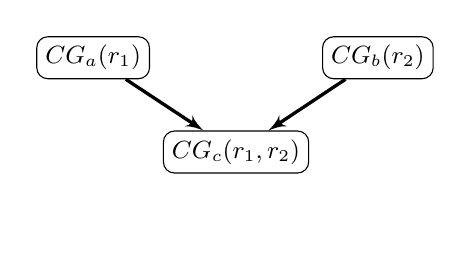
\begin{tikzpicture}[auto] \small
\tikzset{
  Base/.style={align=center}, %, minimum height=2ex},
  Line/.style={draw, very thick, >=latex', black},
  CommandGroup/.style={draw, Base, rounded corners, black},
  Notice/.style  = { draw, above, rounded corners, rectangle callout, text width=6cm,
    callout absolute pointer={#1} },
    }

\matrix (binmat) [ampersand replacement=\&, column sep=0.5em, row sep=2em]
{
  \node [CommandGroup] (CGA)  {$CG_a(r_1)$}; \& 
    \node (empty) {};  \& 
    \node [CommandGroup] (CGB)  {$CG_b(r_2)$}; \\

    \& \node [CommandGroup] (CGC)  {$CG_c(r_1,r_2)$}; \\
    \& \node (empty) {}; \\
};

\path [Line, ->] (CGA) -- (CGC);
\path [Line, ->] (CGB) -- (CGC);
\end{tikzpicture}

\end{multicols}

\caption{Execution order of three command groups submitted to the different
  queues}
\label{fig:three-cg-three-queue}
\end{figure}

\subsection{SYCL Kernel Execution Model}

When a kernel is submitted for execution an index space is defined.
An instance of the kernel body executes for each point in this index space.
This kernel instance is called a \gls{work-item} and is identified by its
point in the index space, which provides a \gls{global-id} for the work-item.  Each
work-item executes the same code but the specific execution pathway through the
code and the data operated upon can vary by using the work-item global id to
specialize the computation.

Work-items are organized into work-groups. The \glspl{work-group} provide a more
coarse-grained decomposition of the index space.  Each work-group is assigned a
unique \gls{work-group-id} with the same dimensionality as the index space used for
the work-items. Work-items are each assigned a \gls{local-id}, unique within the
work-group, so that a single work-item can be uniquely identified by its global
id or by a combination of its local id and work-group id.  The work-items in a
given work-group execute concurrently on the processing elements of a single
compute unit.

The index space supported in SYCL is called an \gls{nd-range}.  An ND-range is an
\textit{N}-dimensional index space, where \textit{N} is one, two or three.  In
SYCL, the ND-range is represented via the \codeinline{nd_range<N>} class.  An
\codeinline{nd_range<N>} is made up of a global range and a local range, each
represented via values of type \codeinline{range<N>} and a global offset,
represented via a value of type \codeinline{id<N>}.  The types
\codeinline{nd_range<N>} and \codeinline{id<N>} are each \textit{N}-element
arrays of integers.  The iteration space defined via an \codeinline{range<N>}
is an \textit{N}-dimensional index space starting at the ND-range's global
offset and being of the size of its global range, split into work-groups of the
size of its local range.

Each work-item in the ND-range is identified by a value of type
\codeinline{nd_item<N>}.  The type \codeinline{nd_item<N>} encapsulates a
global id, local id and work-group id, all of type \codeinline{id<N>},
the iteration space offset also of type \codeinline{id<N>}, as well as
global and local ranges and synchronization operations necessary to
make work-groups useful. Work-groups are assigned ids using a similar
approach to that used for work-item global ids.  Work-items are
assigned to a work-group and given a local id with components in the
range from zero to the size of the work-group in that dimension minus
one.  Hence, the combination of a work-group id and the local id
within a work-group uniquely defines a work-item.

SYCL allows a simplified execution model in which the work-group size
is left unspecified. A kernel invoked over a \codeinline{range<N>},
instead of an \codeinline{nd_range<N>} is executed within an iteration
space of unspecified workgroup size. In this case, less information is
available to each work-item through the simpler \codeinline{item<N>}
class.

\section{Memory Model}
\label{sec:memory.model}

Since SYCL is a single-source programming model, the memory model affects both
the Application and the Device Kernel parts of a program.
On the SYCL Application, the SYCL Runtime will make sure data is available
for execution of the kernels. 
On the SYCL Device kernel, OpenCL rules are mapped to SYCL constructs
to provide the same capabilities using C++ kernels.

\subsection{SYCL Application Memory Model}
\label{sub.section.memmodel.app}

The application running on the host uses SYCL \gls{buffer} objects using instances of
the \codeinline{cl::sycl::buffer} class to allocate memory in the global address
space, or can allocate specialized image memory using the
\codeinline{cl::sycl::image} class. 
In OpenCL, a memory object is attached to a specific context. 

In the SYCL Application, memory objects are bound to all devices in which
they are used, regardless of the SYCL context where they reside.
SYCL memory objects (namely, \gls{buffer} and \gls{image} objects) 
can encapsulate multiple underlying OpenCL memory objects together with
multiple host memory allocations to enable the same object to be shared
between devices in different contexts or platforms.

The order of execution of \gls{command-group} objects ensures a sequentially
consistent access to the memory from the different devices to the memory
objects.

To access memory objects from inside a kernel, the user must create an
\gls{accessor} object which parameterizes the type of access
the kernel requires. 
The \gls{accessor} object defines a requirement to access a memory
object from a \gls{command-group}. 
The \codeinline{cl::sycl::accessor} object specifies
whether the access is via global memory, constant memory or image samplers and
their associated access functions. The \gls{accessor} also specifies whether the
access is read-only (RO), write-only (WO) or read-write (RW). 
An optional \keyword{discard}
flag can be added to an accessor to tell the system to discard any previous
contents of the data the accessor refers to, e.g.\ discard write-only (DW). 
Atomic access can also be requested
on an accessor which allows \codeinline{cl::sycl::atomic} classes to be used via
the accessor.
For simplicity, when a \textbf{requisite} represents an accessor object  in 
a certain access mode, we represent it as 
$\text{MemoryObject}_{\text{AccessMode}}$.
For example, an accessor that accesses memory object \textbf{buf1} in \textbf{RW} 
mode is represented as $buf1_{RW}$.
A \gls{command-group} object that uses such an accessor is represented 
as $CG(buf1_{RW})$.
The \textbf{action} required to satisfy
a requisite and the location 
of the latest copy of a memory object will vary depending on the implementation.

Figure~\ref{fig:devicetodevice} 
illustrates an example where \gls{command-group}
objects are enqueued to two separate SYCL queues executing in devices in
different contexts.
The \textbf{requisites} for the \gls{command-group} execution are 
the same, but the \textbf{actions} to satisfy them are different.
For example, if the data is on the host before execution, 
$A(b1_{RW})$ and $A(b2_{RW})$ can potentially be implemented as copy 
operations from the host memory to \codeinline{context1} or \codeinline{context2}
respectively.
After $CG_a$ and $CG_b$ are executed, $A'(b1_{RW})$ will likely
be an empty operation, since the result of the kernel can stay on the device.
On the other hand, the results of $CG_b$ are now on a different
context than $CG_c$ is executing, therefore $A'(b2_{RW})$ will need to 
copy data across two separate OpenCL contexts using an implementation 
specific mechanism.

\begin{figure}[h]
\centering
\begin{multicols}{2}

\textbf{SYCL Application Enqueue Order}
\vspace{1cm}

\flushleft
{
\fontfamily{qcr}\selectfont
cl::sycl::queue q1(context1);
cl::sycl::queue q2(context2);
q1.submit($CG_a(b1_{RW})$);
q2.submit($CG_b(b2_{RW})$);
q1.submit($CG_c(b1_{RW},b2_{RW})$);
}
\columnbreak

\textbf{SYCL Kernel Execution Order}
\vspace{1cm}

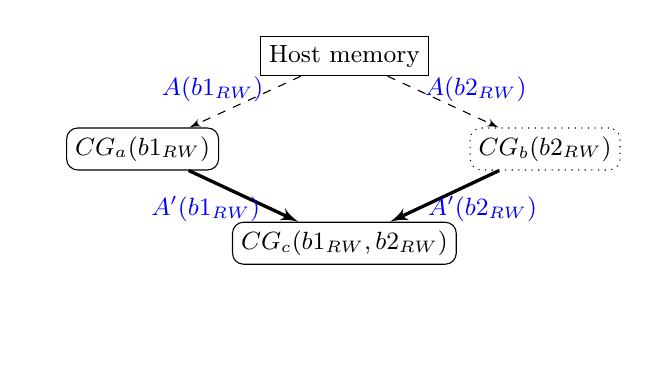
\begin{tikzpicture}[auto] \small
\tikzset{Base/.style={align=center}, %, minimum height=2ex},
  Line/.style={draw, very thick, >=latex', black},
  LineHost/.style={draw, dashed, >=latex', black},
  MemoryObject/.style={draw, Base, black},
  CommandGroup/.style={draw, Base, rounded corners, black},
  Notice/.style  = {draw, above, rounded corners, rectangle callout, text width=6cm,
    callout absolute pointer={#1} },
  Action/.style = {very thick, solid, draw, rectangle callout, rounded corners, black, Base}
    }

\matrix (binmat) [ampersand replacement=\&, column sep=0.5em, row sep=2em]
  {\node  (empty) {}; \& 
    \node (empty) {};  \& 
    \node [MemoryObject] (Host) {Host memory};  \&
    \node (empty) {};  \\
    \node (empty) {};  \&
    \node [CommandGroup] (CGA)  {$CG_a(b1_{RW})$}; \& 
    \node (empty) {};  \& 
    \node [CommandGroup, style=dotted] (CGB)  {$CG_b(b2_{RW})$}; \\
    \node (empty) {};  \&
    \& \node [CommandGroup] (CGC)  {$CG_c(b1_{RW},b2_{RW})$}; \\
    \node (empty) {};  \&
    \& \node (empty) {}; \\
};
  \path [LineHost, ->] (Host) -- node[blue, left=0.2, near start] {$A(b1_{RW})$} (CGA);
  \path [LineHost, ->] (Host) -- node[blue, right=0.2, near start] {$A(b2_{RW})$} (CGB);
  \path [Line, ->] (CGA) -- node[blue, left=0.2, near end] {$A'(b1_{RW})$} (CGC);
  \path [Line, ->] (CGB) -- node[blue, right=0.2, near end] {$A'(b2_{RW})$} (CGC);
\end{tikzpicture}

\end{multicols}

\textbf{Possible implementation by a SYCL Runtime}
\vspace{1cm}

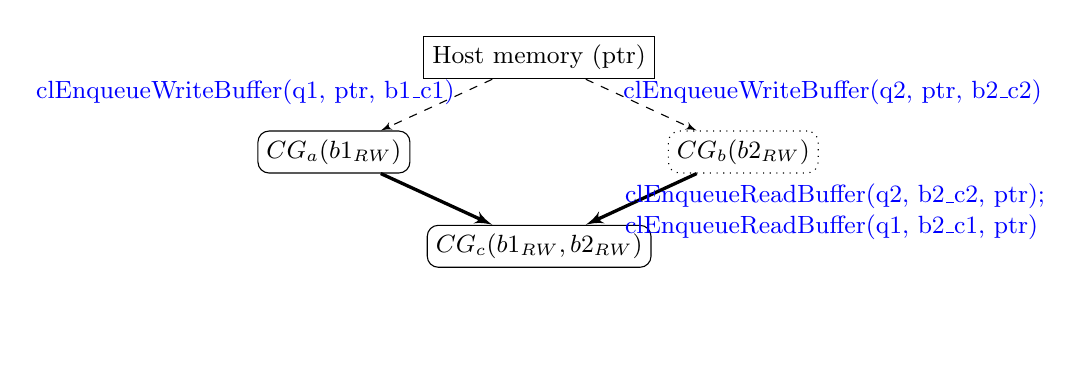
\begin{tikzpicture}[auto] \small
\tikzset{Base/.style={align=center}, %, minimum height=2ex},
  Line/.style={draw, very thick, >=latex', black},
  LineHost/.style={draw, dashed, >=latex', black},
  MemoryObject/.style={draw, Base, black},
  CommandGroup/.style={draw, Base, rounded corners, black},
  Notice/.style  = {draw, above, rounded corners, rectangle callout, text width=6cm,
    callout absolute pointer={#1} },
  Action/.style = {very thick, solid, draw, rectangle callout, rounded corners, black, Base}
    }

\matrix (binmat) [ampersand replacement=\&, column sep=0.5em, row sep=2em]
  {\node  (empty) {}; \& 
    \node (empty) {};  \& 
    \node [MemoryObject] (Host) {Host memory (ptr)};  \&
    \node (empty) {};  \\
    \node (empty) {};  \&
    \node [CommandGroup] (CGA)  {$CG_a(b1_{RW})$}; \& 
    \node (empty) {};  \& 
    \node [CommandGroup, style=dotted] (CGB)  {$CG_b(b2_{RW})$}; \\
    \node (empty) {};  \&
    \& \node [CommandGroup] (CGC)  {$CG_c(b1_{RW},b2_{RW})$}; \\
    \node (empty) {};  \&
    \& \node (empty) {}; \\
};
  \path [LineHost, ->] (Host) -- node[blue, left=0.3, near start] {clEnqueueWriteBuffer(q1, ptr, b1\_c1)} (CGA);
  \path [LineHost, ->] (Host) -- node[blue, right=0.3, near start] {clEnqueueWriteBuffer(q2, ptr, b2\_c2)} (CGB);
  \path [Line, ->] (CGA) -- node[blue, left=0.2, near end] {} (CGC);
  \path [Line, ->] (CGB) -- node[blue, right=0.5, near end, align=left] {clEnqueueReadBuffer(q2, b2\_c2, ptr);\\ clEnqueueReadBuffer(q1, b2\_c1, ptr)} (CGC);
\end{tikzpicture}



\caption{Actions performed when three command groups are submitted 
to two distinct queues, and possible OpenCL implementation of them by
  a SYCL runtime. Note that each SYCL buffer ($b1,b2$) is implemented as
  separate \codeinline{cl_mem} objects per context}
\label{fig:devicetodevice}
\end{figure}

Note that the order of the definition of the accessors within the 
\gls{command-group} is irrelevant to the requirements they define.
All accessors always apply to the entire \gls{command-group} object where
they are defined.
When multiple \glspl{accessor} in the same \gls{command-group} define requirements to the same memory object, the access mode is resolved as the union of
all the different access modes, e.g. $CG(b1_{R},b1_{W})$ is equivalent
to $CG(b1_{RW})$.

A buffer created from a range of an existing buffer is called
a \keyword{sub-buffer}.
A buffer may be overlaid with any number of sub-buffers.
Accessors can be created to operate on these \keyword{sub-buffers}. 
Refer to~\ref{subsec:buffers} for details on \keyword{sub-buffer} 
creation and restrictions.
A requirement to access a sub-buffer is represented by specifying its
range, e.g. $CG(b1_{RW,[0,5)})$ represents the requirement of accessing
the range $[0,5)$ buffer $b1$ in read write mode.

If two accessors are constructed to
access the same buffer, but both are to non-overlapping sub-buffers of the
buffer, then the two accessors are said to not \keyword{overlap}, otherwise the
accessors do overlap. Overlapping is the test that is used to determine the
scheduling order of command groups. 
Command-groups with non-overlapping requirements may execute concurrently.

\begin{figure}[h]
\centering
[tikz,"overlap"]
----
\usetikzlibrary{arrows}
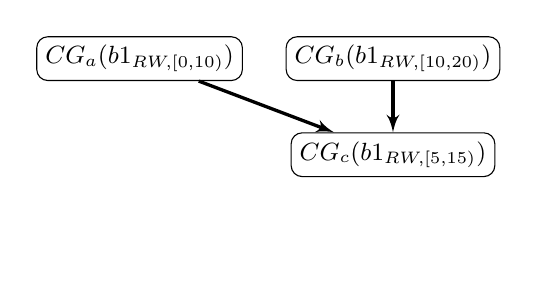
\begin{tikzpicture}[auto] \small
\tikzset{Base/.style={align=center}, %, minimum height=2ex},
  Line/.style={draw, very thick, >=latex', black},
  LineHost/.style={draw, dashed, >=latex', black},
  MemoryObject/.style={draw, Base, black},
  CommandGroup/.style={draw, Base, rounded corners, black},
  Notice/.style  = {draw, above, rounded corners, rectangle callout, text width=6cm,
    callout absolute pointer={#1} },
    }

\matrix (binmat) [ampersand replacement=\&, column sep=0.5em, row sep=2em]
{
    \node [CommandGroup] (CGA) {$CG_a(b1_{RW, [0,10)})$}; \&
    \node (empty) {};  \&
    \node [CommandGroup] (CGB) {$CG_b(b1_{RW, [10, 20)})$}; \\
    \node (empty) {};  \&
    \& \node [CommandGroup] (CGC) {$CG_c(b1_{RW, [5, 15)})$}; \\
    \node (empty) {};  \&

    \& \node (empty) {}; \\
};
\path [Line, ->] (CGA) -- (CGC);
\path [Line, ->] (CGB) -- (CGC);
\end{tikzpicture}
----

\caption{Requirements on overlapping vs non-overlapping \keyword{sub-buffer}}
\label{fig:overlap}
\end{figure}

It is permissible for command groups that only read data to not copy that data
back to the host or other devices after reading and for the runtime to maintain
multiple read-only copies of the data on multiple devices.

A special case of requirement is the one defined by a \textbf{host accessor}.
Host accessors are represented with $H(\text{MemoryObject}_{\text{accessMode}})$, e.g,
$H(b1_{RW})$ represents a host accessor to $b1$ in read-write mode.
Host accessors are a special type of accessor constructed from a memory
object outside a command group, and require that the data associated with
the given memory object is available on the host in the given pointer.
This causes the runtime to block on construction of this object until the
requirement has been satisfied. 
\textbf{Host accessor} objects are effectively barriers on all accesses to 
a certain memory object.
Figure~\ref{fig:host-acc} shows an example of multiple command groups
enqueued to the same queue. Once the host accessor $H(b1_{RW})$ is reached,
the execution cannot proceed until $CG_a$ is finished. 
However, $CG_b$ does not have any requirements on $b1$, therefore, it can
execute concurrently with the barrier.
Finally, $CG_c$ will be enqueued after $H(b1_{RW})$ is finished, 
but still has to wait for $CG_b$ to conclude for all its requirements to
be satisfied.
See~\ref{sec:synchronization} for details on synchronization rules.

\begin{figure}[h]
\centering
% Copyright (c) 2012-2019 Khronos Group.
%
% This work is licensed under a Creative Commons Attribution 4.0
% International License.
% http://creativecommons.org/licenses/by/4.0/

\begin{multicols}{2}

\textbf{SYCL Application Enqueue Order}
\vspace{1cm}

\newcommand{\cga}{$CG_a(b1_{RW})$}
\newcommand{\cgb}{$CG_b(b2_{RW})$}
\newcommand{\hostA}{$H(b1_{RW})$}
\newcommand{\cgc}{$CG_c(b1_{RW}, b2_{RW})$}

\flushleft
{
\fontfamily{qcr}\selectfont
cl::sycl::queue q1;
q1.submit(\cga);
q1.submit(\cgb);

\hostA;

q1.submit(\cgc);
}
\columnbreak

\textbf{SYCL Kernel Execution Order}
\vspace{1cm}

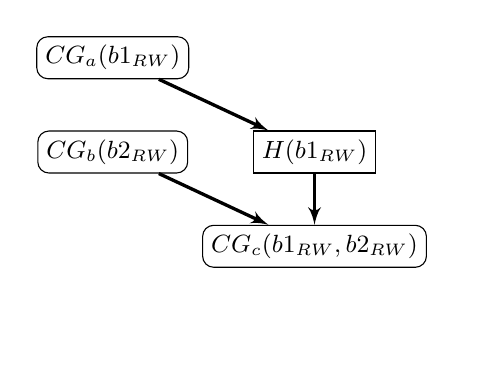
\begin{tikzpicture}[auto] \small
\tikzset{Base/.style={align=center}, %, minimum height=2ex},
  Line/.style={draw, very thick, >=latex', black},
  LineHost/.style={draw, dashed, >=latex', black},
  MemoryObject/.style={draw, Base, black},
  HostAcc/.style={draw, Base, black, cylinder},
  CommandGroup/.style={draw, Base, rounded corners, black},
  Notice/.style  = {draw, above, rounded corners, rectangle callout, text width=6cm,
    callout absolute pointer={#1} },
    }

\matrix (binmat) [ampersand replacement=\&, column sep=0.5em, row sep=2em]
{
    \node [CommandGroup] (CGA)  {\cga}; \& 
    \node (empty) {};  \& 
    \node (empty) {};  \\
    \node [CommandGroup] (CGB)  {\cgb}; \&
    \node [MemoryObject] (HA) {\hostA};  \\
    \& \node [CommandGroup] (CGC)  {\cgc}; \\
    \node (empty) {};  \&

    \& \node (empty) {}; \\
};
\path [Line, ->] (CGA) -- (HA);
\path [Line, ->] (CGB) -- (CGC);
\path [Line, ->] (HA) -- (CGC);
\end{tikzpicture}

\end{multicols}

\caption{Execution of command groups when using host accessors}
\label{fig:host-acc}
\end{figure}

\subsection{SYCL Device Memory Model}

The Memory Model for SYCL Devices is based on the OpenCL Memory model.
Work-items executing in a kernel have access to four distinct memory regions:

\begin{itemize}
    \item \Gls{global-memory} is accessible to all work-items in all
work-groups. Work-items can read from or write to any element of a global memory
object. Reads and writes to global memory may be cached depending on the
capabilities of the device. Global memory is persistent across kernel
invocations, however there is no guarantee that two concurrently executing
kernels can simultaneously write to the same memory object and expect correct
results.

    \item \Gls{constant-memory} is a region of global memory that remains
constant during the execution of a kernel. The host allocates and initializes
memory objects placed into constant memory.

    \item \Gls{local-memory} is a distinct memory region shared between
work-items in a single work-group and inaccessible to work-items in other
work-groups. This memory region can be used to allocate variables that are
shared by all work-items in a work-group. Work-group-level visibility allows
local memory to be implemented as dedicated regions of memory on an OpenCL
device where this is appropriate.

    \item \Gls{private-memory} is a region of memory private to a work-item.
Variables defined in one work-item's private memory are not visible to another
work-item.
\end{itemize}

\subsubsection{Access to memory}

Accessors in the device kernels provide access to the memory objects, 
acting as pointers to the corresponding address space.

It is not possible to pass a pointer into host memory directly as a kernel
parameter because the devices may be unable to support the same address space
as the host.

To allocate local memory within a kernel, the user can either pass
a \codeinline{cl::sycl::local_accessor} object to the kernel as a parameter, or
can define a variable in workgroup scope inside
\codeinline{cl::sycl::parallel_for_work_group}.

Any variable defined inside a \codeinline{cl::sycl::parallel_for} scope or
\codeinline{cl::sycl::parallel_for_work_item} scope will be allocated in private
memory. Any variable defined inside a \codeinline{cl::sycl::parallel_for_work_group}
scope will be allocated in local memory.

Users can create accessors that reference sub-buffers as well as entire buffers.

Within kernels, the underlying C++ pointer types can be obtained from an
accessor. The pointer types will contain a compile-time deduced address space.
So, for example, if a C++ pointer is obtained from an accessor to global memory, 
the C++ pointer type will have a global address space attribute attached to it. 
The address space attribute will be compile-time propagated to other pointer
values when one pointer is initialized to another pointer value using a defined
mechanism.

When developers need to explicitly state the address space of a pointer value,
one of the explicit pointer classes can be used. There is a different explicit
pointer class for each address space: \codeinline{cl::sycl::local_ptr},
\codeinline{cl::sycl::global_ptr}, \codeinline{cl::sycl::private_ptr},
or \codeinline{cl::sycl::constant_ptr}. An accessor declared with one
address space can be implicitly cast to an explicit pointer class
for the same address space. Explicit pointer class values cannot be passed
as parameters to kernels or stored in global memory.


For templates that need to adapt to different address spaces, a
\codeinline{cl::sycl::multi_ptr} class is defined which is templated
via a compile-time constant enumerator value to specify the address space.

\subsubsection{Memory consistency}

OpenCL uses a relaxed memory consistency model, i.e.\ the state of
memory visible to a work-item is not guaranteed to be consistent
across the collection of work-items at all times. This also applies to
SYCL kernels.

As in OpenCL, within a work-item memory has load/store consistency. Both local
memory and global memory may be made consistent across work-items in a single
work-group through use of a \gls{work-group-barrier} or \gls{work-group-mem-fence} operation with appropriate flags. There are no guarantees of memory consistency between different work-groups executing a kernel or between different kernels during their execution.

\subsubsection{Atomic operations}

Atomic operations can be performed on memory in buffers. The range of
atomic operations available on a specific OpenCL device is limited by
the atomic capabilities of that device.  The
\codeinline{cl::sycl::atomic<T>} must be used for elements of a buffer
to provide safe atomic access to the buffer from device code.

\section{The SYCL programming model}

SYCL programs are explicitly parallel and expose the full heterogeneous
parallelism of the underlying machine model of OpenCL. This includes exposing
the data-parallelism, multiple execution devices and multiple memory storage
spaces of OpenCL. However, SYCL adds on top of OpenCL a higher level of
abstraction allowing developers to hide much of the complexity from the source
code, when a developer so chooses.

A SYCL program is written in standard C++. Host code and device code is
written in the same C++ source file, enabling instantiation of templated
kernels from host code and also enabling kernel source code to be shared
between host and device.
The device kernels are encapsulated C++ function objects (a
type callable with \codeinline{operator()} or a lambda function), which have
been designated to be compiled as SYCL kernels. SYCL will
also accept OpenCL \codeinline{cl_kernel} objects.

SYCL programs target heterogeneous systems. The kernels may be compiled and
optimized for multiple different processor architectures with very different
binary representations.

The C++ features used in SYCL are a subset of the C++11 standard features.
Users will need to compile SYCL source code with C++ compilers which support
the following C++ features:
\begin{itemize}
\item All C++03 features, apart from Run Time Type Information
\item Exception handling
\item C++11 lambda functions
\item C++11 variadic templates
\item C++11 template aliases
\item C++11 rvalue references
\item C++11 \codeinline{std::function}, \codeinline{std::string} and
  \codeinline{std::vector}.
\end{itemize}

\subsection{Basic data parallel kernels} 

Data-parallel kernels that execute as
multiple work-items and where no local synchronization is required are enqueued
with the \codeinline{cl::sycl::parallel_for} function parameterized by a
\codeinline{cl::sycl::range} parameter. These kernels will execute the kernel
function body once for each work-item in the range. The range passed to
\codeinline{cl::sycl::parallel_for} represents the global size of an OpenCL
kernel and will be divided into work-groups whose size is chosen by the SYCL
runtime. Barrier synchronization is not valid within these work-groups.

\subsection{Work-group data parallel kernels}

Data parallel kernels can also execute in a mode where the set of
work-items is divided into work-groups of user-defined dimensions.
The user specifies the global range and local work-group size as
parameters to the \codeinline{cl::sycl::parallel_for} function with a
\codeinline{cl::sycl::nd_range} parameter. In this mode of execution,
kernels execute over the nd_range in work-groups of the specified
size. It is possible to share data among work-items within the same
work-group in local or global memory and to synchronize between
work-items in the same work-group by calling the 
\codeinline{nd_item::barrier()} function. All work-groups in a given
\codeinline{parallel_for} will be the same size and the global size
defined in the nd_range must be a multiple of the work-group size in
each dimension.

\subsection{Hierarchical data parallel kernels}

The SYCL compiler provides a way of specifying data parallel kernels
that execute within work-groups via a different syntax which
highlights the hierarchical nature of the parallelism. This mode is
purely a compiler feature and does not change the execution model of
the kernel. Instead of calling \codeinline{cl::sycl::parallel_for} the
user calls \codeinline{cl::sycl::parallel_for_work_group} with a
\codeinline{cl::sycl::range} value representing the number of
work-groups to launch and optionally a second
\codeinline{cl::sycl::range} representing the size of each work-group
for performance tuning. All code within the
\codeinline{parallel_for_work_group} scope effectively executes once
per work-group. Within the \codeinline{parallel_for_work_group} scope,
it is possible to call \codeinline{parallel_for_work_item} which
creates a new scope in which all work-items within the current
work-group execute. This enables a programmer to write code that looks
like there is an inner work-item loop inside an outer work-group loop,
which closely matches the effect of the execution model. All variables
declared inside the \codeinline{parallel_for_work_group} scope are
allocated in workgroup local memory, whereas all variables declared
inside the \codeinline{parallel_for_work_item} scope are declared in
private memory. All \codeinline{parallel_for_work_item} calls within a
given \codeinline{parallel_for_work_group} execution must have the
same dimensions.


\subsection{Kernels that are not launched over parallel instances}

Simple kernels for which only a single instance of the kernel function will be
executed are enqueued with the \codeinline{cl::sycl::single_task} function. The
kernel enqueued takes no ``work-item id'' parameter and will only execute once.
The behavior is logically equivalent to executing a kernel on a single compute
unit with a single work-group comprising only one work-item. Such kernels may be
enqueued on multiple queues and devices and as a result may, like any other
OpenCL entity, be executed in task-parallel fashion.

\subsection{Synchronization}
\label{sec:synchronization}

Synchronization of processing elements executing inside a device is handled
by the SYCL device kernel following OpenCL rules.
The synchronization of the different SYCL device kernels executing with 
the host memory is handled by the SYCL Application via the SYCL runtime.

\subsubsection{Synchronization in the SYCL Application}

Synchronization points between host and device(s) are exposed through 
the following operations:

\begin{itemize}
  \item
    \emph{Buffer destruction}: The destructors for
    \codeinline{cl::sycl::buffer} and \codeinline{cl::sycl::image}
    objects wait for all submitted work on those objects to complete
    and copies the data back to host memory before returning, if there
    is anything to copy back to the host or if the objects were
    constructed with attached host memory.

    More complex forms of synchronization on buffer destruction
    can be specified by the user by constructing buffers with other kinds of
    references to memory, such as \tf{shared_ptr} and \tf{unique_ptr}.
  \item
    \emph{Host Accessors}: The constructor for a host accessor waits for
    all kernels that modify the same buffer (or image) in any queues to complete
    and then copies data back to host memory before the constructor returns. Any
    command groups with requirements to the same memory object cannot execute
    until the host accessor is destroyed (see~\ref{fig:host-acc}).
  \item
    \emph{Command group enqueue}: The \gls{sycl-runtime} internally ensures that
    any command groups added to queues have the correct event dependencies added
    to those queues to ensure correct operation. Adding command groups to queues
    never blocks. Instead any required synchronization is added to the queue and
    events of type \codeinline{cl::sycl::event} are returned by the queue's submit
    function that contain event information related to the specific command
    group.
  \item 
    \emph{Queue operations}: The user can manually use queue operations, such
    as \textbf{wait} to block execution of the caller thread until all the
    command groups submitted to the queue have finished execution. Note that
    this will also affect the dependencies of those command groups in other
    queues.
  \item
    \emph{Interaction with OpenCL synchronization operations}: The user can
    obtain OpenCL events from command groups which will
    enable the user to add \glspl{barrier} to their own queues to correctly
    synchronize for buffer or image data dependencies.
  \item
   \emph{SYCL event objects}: SYCL provides \codeinline{cl::sycl::event} objects
   which can be used for user synchronization. If synchronization is required
   between two different OpenCL contexts, then the \gls{sycl-runtime} ensures that
   any extra host-based synchronization is added to enable the SYCL event
   objects to operate between contexts correctly.

 \end{itemize}

Note that the destructors of other SYCL objects
(\codeinline{cl::sycl::queue}, \codeinline{cl::sycl::context}\ldots) do
not block. Only a \codeinline{cl::sycl::buffer} or
\codeinline{cl::sycl::image} destructor might block. The rationale is
that an object without any side effect on the host does not need to
block on destruction as it would impact the performance. So it is up
to the programmer to use a method to wait for completion in some
cases if this does not fit the goal.
See Section~\ref{sec:managing-object-lifetimes} for more information
on object life time.

\subsubsection{Synchronization in SYCL Kernels}

In SYCL, synchronization can be either global or local within a
\gls{work-group}.  The SYCL implementation may need to provide extra
synchronization commands and host-side synchronization in order to
enable synchronization across OpenCL contexts, but this is handled
internally within the \gls{sycl-runtime}.

Synchronization between work-items in a single work-group is achieved
using a \gls{work-group-barrier}. This matches the OpenCL C behavior. All
the work-items of a work-group must execute the barrier before any are
allowed to continue execution beyond the barrier. Note that the
work-group barrier must be encountered by all work-items of a
work-group executing the kernel or by none at all. There is no
mechanism for synchronization between work-groups. In SYCL, work-group
barriers are exposed through the method on the
\codeinline{cl::sycl::nd_item} class, \codeinline{nd_item::barrier()}
which is only available inside
kernels that are executed over work-groups. This ensures that
developers can only use work-group barriers inside work-groups.

\subsection{Error handling}

In SYCL, there are two types of error: synchronous errors that can be
detected immediately, and asynchronous errors that can only be
detected later.  Synchronous errors, such as failure to construct an
object, are reported immediately by the runtime throwing an
exception. Asynchronous errors, such as an error occurring during
execution of a kernel on a device, are reported via user-supplied
asynchronous error-handlers.

A \codeinline{cl::sycl::context} can be constructed with a
user-supplied asynchronous error handler. If a \codeinline{cl::sycl::queue}
is constructed without a user-supplied context, then the user can supply
an asynchronous error handler for the queue, otherwise errors on that
queue will be reported to its context error handler.

Asynchronous errors are not reported immediately as they occur. The
asynchronous error handler for a context or queue is called with a
\codeinline{cl::sycl::exception_list} object, which contains a list of
asynchronously-generated exception objects, either on destruction of
the context or queue that the error handler is associated with, or via
an explicit \codeinline{wait_and_throw} method call on an associated
queue. 

\subsection{Fallback Mechanism}

A \gls{command-group-function-object} can be submitted either to a single queue 
to be executed on, or to a secondary queue. If a
\gls{command-group-function-object} fails to be enqueued to the primary queue, then
the system will attempt to enqueue it to the secondary queue, if given as a
parameter to the submit function. If the \gls{command-group-function-object} fails to be
queued to both of these queues, then a synchronous SYCL exception will be thrown.

It is possible that a command group may be successfully enqueued,
but then asynchronously fail to run, for some reason. In this case, it may be
possible for the runtime system to execute the \gls{command-group-function-object}
on the secondary queue, instead of the primary queue. The situations where a SYCL
runtime may be able to achieve this asynchronous fall-back is implementation-defined.

\subsection{Scheduling of kernels and data movement}

A \gls{command-group-function-object} takes a reference to a command group
\codeinline{handler} as a parameter and anything within that scope is
immediately executed and has to get the handler object as a parameter. The
intention is that a user will perform calls to SYCL functions, methods,
destructors and constructors inside that scope. These calls will be non-blocking
on the host, but enqueue operations to the queue that the command group is submitted
to. All user functions within the command group scope will be called on the host
as the \gls{command-group-function-object} is executed, but any runtime SYCL
operations will be queued.

It is worth noting that a SYCL queue does not necessarily map to only one OpenCL
queue, however, the OpenCL queue that is given when interacting with the SYCL
queue will retain any synchronization information that is needed for synchronization
with any other OpenCL queues spawned by the system.

An OpenCL implementation can require different queues for different devices and
contexts. The synchronization required to ensure order between commands in
different queues varies according to whether the queues have shared contexts.
A SYCL implementation must determine the required synchronization to ensure the
above ordering rules above are enforced.

\subsection{Managing object lifetimes}
\label{sec:managing-object-lifetimes}

SYCL does not initialize any OpenCL features until a
\codeinline{cl::sycl::context} object is created. A user does not need to
explicitly create a \codeinline{cl::sycl::context} object, but they do need to
explicitly create a \codeinline{cl::sycl::queue} object, for which a
\codeinline{cl::sycl::context} object will be implicitly created if not provided
by the user.

All OpenCL objects encapsulated in SYCL objects are reference-counted and will
be destroyed once all references have been released. This means that a user needs
only create a SYCL queue (which will automatically create an OpenCL context) for
the lifetime of their application to initialize and release the OpenCL context
safely.

When an OpenCL object that is encapsulated in a SYCL object is copied in C++,
then the underlying OpenCL object is not duplicated, but its OpenCL reference
count is incremented. When the original or copied SYCL object is destroyed, then
the OpenCL reference count is decremented.

There is no global state specified to be required in SYCL implementations. This
means, for example, that if the user creates two queues without explicitly
constructing a common context, then a SYCL implementation does not have to
create a shared context for the two queues. Implementations are free to share or
cache state globally for performance, but it is not required.

Memory objects can be constructed with or without attached host memory. If no
host memory is attached at the point of construction, then destruction of that
memory object is non-blocking. The user may use C++ standard pointer classes
for sharing the host data with the user application and for defining blocking,
or non-blocking behavior of the buffers and images.
If host memory is attached by using a raw pointer,  then the default behavior is
followed, which is that the destructor will block until any command groups
operating on the memory object have completed, then, if the contents of the
memory object is modified on a device those contents are copied back to host and
only then does the destructor return. Instead of a raw pointer, a
\codeinline{unique_ptr} may be provided, which uses move semantics for initializing
and using the associated host memory. In this case, the behavior of the buffer
in relation to the user application
will be non-blocking on destruction. In the case where host memory is shared
between the user application and the \gls{sycl-runtime}, then the reference counter
of the \codeinline{shared_ptr} determines whether the buffer needs to copy
data back on destruction, and in that case the blocking or non-blocking behavior
depends on the user application.


As said in Section~\ref{sec:synchronization}, the only blocking
operations in SYCL (apart from explicit wait operations) are:
\begin{itemize}
\item host accessor constructor, which waits for any kernels enqueued before
its creation that write to the corresponding object to finish and be copied back
to host memory before it starts processing. The host accessor does not
necessarily copy back to the same host memory as initially given by the
user;
\item memory object destruction, in the case where copies back to host memory
have to be done or when the host memory is used as a backing-store.
\end{itemize}
\todo{RK: this list seems very similar to what is said in
  Section~\ref{sec:synchronization}, where the platform destruction seems
  to be forgotten. This is logical since we use RAII. But even it is not
  possible to factorize some text, at least the 2 sections should be
  cross-referenced}


\subsection{Device discovery and selection}

A user specifies which queue to submit a \gls{command-group-function-object} on and
each queue is targeted to run on a specific device (and context). A user can specify
the actual device on queue creation, or they can specify a \keyword{device selector}
which causes the \gls{sycl-runtime} to choose a device based on the user's provided
preferences. Specifying a selector causes the \gls{sycl-runtime} to perform device
discovery. No device discovery is performed until a SYCL selector is passed to a
queue constructor. Device topology may be cached by the \gls{sycl-runtime}, but this
is not required.

Device discovery will return both OpenCL devices and platforms as well as a
SYCL host platform and SYCL host device. The host device allows queue creation
and running of kernels, but does not support OpenCL-specific features. It is an
error for a user to request an underlying OpenCL device for the SYCL host device.

\subsection{Interfacing with OpenCL}
\label{sec:interfacing-with-opencl}

%https://cvs.khronos.org/bugzilla/show_bug.cgi?id=10426

\gls{sycl-runtime} classes which encapsulate an OpenCL opaque type such as SYCL \codeinline{context} or SYCL \codeinline{queue} must provide an interoperability constructor taking an instance of the OpenCL opaque type.
These constructors must retain that instance to increase the reference count of the OpenCL resource.

\gls{sycl-runtime} classes which encapsulate an OpenCL opaque type (excluding the SYCL \codeinline{buffer} and SYCL \codeinline{image} class templates) can be queried for their encapsulated instance via a \codeinline{get()} member function. These \codeinline{get()} member functions must retain the instance to increase the reference count of the OpenCL resource.

The destructor for the \gls{sycl-runtime} classes which encapsulate an OpenCL opaque type must release that instance to decrease the reference count of the OpenCL resource.

Note that an instance of a \gls{sycl-runtime} class which encapsulates an OpenCL opaque type can encapsulate any number of instances of the OpenCL type, unless it was constructed via the interoperability constructor in which case it may only encapsulate a single instance of that the OpenCL type.

Note that the lifetime of a \gls{sycl-runtime} class that encapsulates an OpenCL opaque type and the instance of that opaque type retrieved via the \codeinline{get()} member function are not tied in either direction given correct usage of OpenCL reference counting. For example if a user were to retrieve a \codeinline{cl_command_queue} instance from a SYCL \codeinline{queue} instance and then immediately destroy the SYCL \codeinline{queue} instance, the \codeinline{cl_command_queue} instance is still valid. Or if a user were to construct a SYCL \codeinline{queue} instance from a \codeinline{cl_command_queue} instance and then immediately release the \codeinline{cl_command_queue} instance, the SYCL \codeinline{queue} instance is still valid.

Note that a \gls{sycl-runtime} class that encapsulates an OpenCL opaque type is not responsible for any incorrect use of OpenCL reference counting outside of the \gls{sycl-runtime}. For example if a user were to retrieve a \codeinline{cl_command_queue} instance from a SYCL \codeinline{queue} instance and then release the \codeinline{cl_command_queue} instance more than once without any prior retain then the SYCL \codeinline{queue} instance that the \codeinline{cl_command_queue} instance was retrieved from is now undefined.

Note that an instance of the SYCL \codeinline{buffer} or SYCL \codeinline{image} class templates constructed via the interoperability constructor is free to copy from the \codeinline{cl_mem} into another memory allocation within the \gls{sycl-runtime} to achieve normal SYCL semantics, for as long as the SYCL \codeinline{buffer} or SYCL \codeinline{image} instance is alive.

\section{Memory objects}

Memory objects in SYCL fall into one of two categories: \gls{buffer} objects
and \gls{image} objects. A buffer object stores a one-, two- or
three-dimensional collection of elements that are stored linearly directly back
to back in the same way C or C++ stores arrays. An image object is used to store
a one-, two- or three-dimensional texture, frame-buffer or image that may be
stored in an optimized and device-specific format in memory and must be accessed
through specialized operations.

Elements of a buffer object can be a scalar data type (such as an int, float),
vector data type, or a user-defined structure. In SYCL, a \gls{buffer} object is a
templated type (\codeinline{cl::sycl::buffer}), parameterized by the element
type and number of dimensions. An \gls{image} object is stored in one of a limited
number of formats. The elements of an image object are selected from a list of
predefined image formats which are provided by an underlying OpenCL
implementation.  Images are encapsulated in the \codeinline{cl::sycl::image}
type, which is templated by the number of dimensions in the image. The minimum
number of elements in a memory object is one.

The fundamental differences between a buffer and an image object are:
\begin{itemize}
    \item
        Elements in a buffer are stored in an array of 1, 2 or 3
        dimensions and can be accessed using an accessor by a kernel
        executing on a device. The accessors for kernels can be
        converted within a kernel into C++ pointer types, or
        the \codeinline{cl::sycl::global_ptr},
        \codeinline{cl::sycl::constant_ptr} classes.
        Elements of an image are
        stored in a format that is opaque to the user and cannot be
        directly accessed using a pointer.  SYCL provides image
        accessors and samplers to allow a kernel to read from or write
        to an image.

      \item For a buffer object the data is accessed within a kernel
        in the same format as it is stored in memory, but in the case
        of an image object the data is not necessarily accessed within
        a kernel in the same format as it is stored in memory.

        Image elements are always a
          4-component vector (each component can be a float or signed/
  unsigned integer) in a kernel.  The SYCL accessor and
        sampler methods to read from an image convert an image element from
          the format that it is stored in to a 4-component vector.  Similarly, the
          SYCL accessor methods provided to write to an image convert the image
          element from a 4-component vector to the appropriate image format
          specified such as 4 8-bit elements, for
        example.  
\end{itemize}

Memory objects, both buffers and images, may have one or more underlying OpenCL
\codeinline{cl_mem} objects. When a buffer or image is allocated on more than
one OpenCL device, if these devices are on separate contexts then multiple
\codeinline{cl_mem} objects may be allocated for the memory object, depending on
whether the object has actively been used on these devices yet or not.


Users may want fine-grained control of the synchronization, memory management
and storage semantics of SYCL image or buffer objects. For example, a user may
wish to specify the host memory for a memory object to use, but may not want the
memory object to block on destruction.

Depending on the control and the use cases of the SYCL applications,
well established C++ classes and patterns can be used for reference counting and
sharing data between user applications and the \gls{sycl-runtime}. For control over
memory allocation on the host and mapping between host and device memory, pre-defined or user-defined C++
\codeinline{allocator} classes are used. For better control of synchronization between a SYCL and a non
SYCL application  that share data, \codeinline{shared_ptr} and \codeinline{mutex}
classes are used. In the case where the user would not like the host side to
block on destruction of buffers or images, as the data given to the buffers are
for initialization only, the \codeinline{unique_ptr} class can be used instead of a
raw pointer to data.

\section{SYCL for OpenCL Framework} 

The SYCL framework allows applications to
use a host and one or more OpenCL devices as a single heterogeneous parallel
computer system. The framework contains the following components:
\begin{itemize}
  \item
    \gls{sycl-library}: The template library provides a
    set of C++ templates and classes which provide the programming model to the
    user. It enables the creation of runtime classes such as SYCL queues,
    buffers and images, as well as access to some underlying OpenCL
    runtime object, such as contexts, platforms, devices and program objects.

  \item 
    \gls{sycl-runtime}: The \gls{sycl-runtime} interfaces with the underlying
    OpenCL implementations and handles scheduling of commands in queues, moving of
    data between host and devices, manages contexts, programs, kernel compilation
    and memory management.

   \item 
     \keyword{OpenCL Implementation(s)}: The SYCL system assumes the existence
     of one or more OpenCL implementations available on the host machine. If no
     OpenCL implementation is available, then the SYCL implementation provides only
     the \gls{host-device} to run kernels on. 
   \item
      SYCL \glspl{device-compiler}: The SYCL \glspl{device-compiler} compile SYCL C++
       kernels into a format which can be executed on an OpenCL device at runtime.
       There may be more than one SYCL device compiler in a SYCL implementation. The
       format of the compiled SYCL kernels is not defined.  A SYCL device compiler may,
       or may not, also compile the host parts of the program.
\end{itemize}

\section{SYCL device compiler}

To enable SYCL to work on a variety of platforms, with different devices,
operating systems, build systems and host compilers, SYCL provides a number of
options to implementers to enable the compilation of SYCL kernels for devices,
while still providing a unified programming model to the user.

\subsection{Building a SYCL program}

A SYCL program runs on a \emph{host} and one or more OpenCL devices. This
requires a compilation model that enables compilation for a variety of targets.
There is only ever one host for the SYCL program, so the compilation of the
source code for the host must happen once and only once. Both kernel and
non-kernel source code is compiled for the host.

The design of SYCL enables a single SYCL source file to be passed to multiple,
different compilers, using the \gls{smcp}
technique. This is an implementation option and is not required.
What this option enables is for an implementer to provide a device compiler only
and not have to provide a host compiler. A programmer who uses such an
implementation will compile the same source file twice: once with the host
compiler of their choice and once with a device compiler. This approach allows
the advantages of having a single source file for both host code and kernels,
while still allowing users an independent choice of host and SYCL device
compilers. 

Only the \glspl{kernel} are compiled for OpenCL devices. Therefore, any compiler that
compiles only for one or more devices must not compile non-kernel source code.
Kernels are contained within C++ source code and may be dependent on lambda
capture and template parameters, so compilation of the non-kernel code must
determine lambda captures and template parameters, but not generate device code
for non-kernel code.

Compilation of a SYCL program may follow either of the following options.
The choice of option is made by the implementer:

\begin{enumerate}
\item
   \keyword{Separate compilation}:
        One or more device compilers compile just the SYCL kernels for one
        or more devices.
        The device compilers all produce header files for interfacing between
        the \gls{host} compiler and the \gls{sycl-runtime},which are integrated 
  together with a tool that produces a single header file.
        The user compiles the source file with a normal C++ host compiler for
        their platform.
        The user must ensure that the host compiler is given the correct
        command-line arguments to ensure that the device
        compiler output header file is \tf{\#include}d from inside the SYCL
        header files.
\item
   \keyword{Single-source compiler}:
    In this approach, a single compiler may compile an entire source file
    for both host and one or more devices.  It is the responsibility of the
    single-source compiler to enable kernels to be compiled correctly for
    devices and enqueued from the host.
 \end{enumerate}

An implementer of SYCL may choose an implementation approach from the options
above.

\subsection{Naming of kernels}

SYCL kernels are extracted from C++ source files and stored in an
implementation-defined format. When the \gls{sycl-runtime} needs to enqueue a SYCL
kernel, it is necessary for the \gls{sycl-runtime} to load the kernel and pass it to an
OpenCL runtime. This requires the kernel to have a globally-visible name to
enable an association between the kernel invocation and the kernel itself. The
association is achieved using a \gls{kernel-name}, which is a C++ type
name.

For a named function object, the kernel name can be the same type as the function object itself,
as long as the function object type is globally accessible. For a lambda function,
there is no globally-visible name, so the user must provide one. In SYCL,
the name is provided as a template parameter to the kernel invocation, e.g.
\codeinline{parallel_for<class kernelName>}.

A device compiler should detect the kernel invocations (e.g.
\codeinline{parallel_for}) in the source code and compile the
enclosed kernels, storing them with their associated type name. For details
please refer to ~\ref{sec:naming.kernels}.
The user can also extract OpenCL \codeinline{cl_kernel} and
\codeinline{cl_program} objects for kernels by providing the type name of the
kernel.



\section{Language restrictions in kernels}

The SYCL \glspl{kernel} are executed on SYCL devices and all of the functions called
from a SYCL kernel are going to be compiled for the device by a SYCL 
\gls{device-compiler}. Due to restrictions of the OpenCL 1.2 runtime and 
OpenCL 1.2 capable
devices, there are certain restrictions for SYCL kernels. Those restrictions can
be summarized as the kernels cannot include RTTI information, exception classes,
recursive code, virtual functions or make use of C++ libraries that are not
compiled for the device. For more details on language restrictions please refer
to~\ref{sec:language.restrictions.kernels}.

SYCL kernels use parameters that are captured by value in the 
\gls{command-group-scope} or are passed from the
host to the device using the data management runtime classes of
\codeinline{cl::sycl::accessors}. Sharing data structures between host and
device code imposes certain restrictions, such as use of only user defined
classes that are \emph{C++11 standard layout} classes for the data structures,
and in general, no pointers initialized for the host can be used on the device. The
only way of passing pointers to a kernel is through the
\codeinline{cl::sycl::accessor} class, which supports the
\codeinline{cl::sycl::buffer} and \codeinline{cl::sycl::image} classes. No
hierarchical structures of these classes are supported and any other data
containers need to be converted to the SYCL data management classes using the
SYCL interface. For more details on the rules for kernel parameter passing,
please refer to~\ref{sec:kernel.parameter.passing}.

Some types in SYCL vary according to pointer size or vary on the host
according to the host ABI, such as \codeinline{size_t} or \codeinline{long}. In order
for the the SYCL device compiler to ensure that the sizes of
these types match the sizes on the host and to enable data of these types
to be shared between host and device, the OpenCL interoperability types
are defined, \codeinline{cl::sycl::cl_int} and \codeinline{cl::sycl::cl_size_t}.

The OpenCL C function qualifier \tf{__kernel} and the access
qualifiers: \tf{__read_only}, \tf{__write_only} and \tf{__read_write}
are not exposed in SYCL via keywords, but are instead encapsulated in
SYCL's parameter passing system inside accessors. Users wishing to
achieve the OpenCL equivalent of these qualifiers in SYCL should
instead use SYCL accessors with equivalent semantics.

\subsection{SYCL Linker}

In SYCL only offline linking is supported for SYCL and OpenCL programs
and libraries, however the mechanism is optional.
In the case of linking C++ functions to a SYCL application,
where the definitions are not available in the
same translation unit of the compiler, then the macro \codeinline{SYCL_EXTERNAL}
has to be provided.
Any OpenCL C function included in a pre-built OpenCL library can be
defined as an \codeinline{extern "C"} function and the OpenCL program
has to be linked against any SYCL program that contains kernels using
the external function. In this case, the data types used have to comply with
the interoperability aliases defined in~\ref{table.types.aliases}.

\subsection{Functions and datatypes available in kernels}


Inside kernels, the functions and datatypes available are restricted by the
underlying capabilities of OpenCL devices. All OpenCL C features are provided
by C++ classes and functions, which are available on host and device.


\section{Execution of kernels on the SYCL host device}

SYCL enables kernels to run on either the host device or on OpenCL devices. When
kernels run on an OpenCL device, then the features and behavior of that
execution follows the OpenCL specification, otherwise they follow the behavior
specified for the \gls{host-device}.

Any kernel enqueued to a host queue executes on the host device according to the
same rules as the OpenCL devices.

Kernel math library functions on the host must conform to OpenCL math precision
requirements. The SYCL host device needs to be queried for the capabilities it provides.

The range of image formats supported by the host device is implementation-defined, 
but must match the minimum requirements of the OpenCL specification.

Some of the OpenCL extensions and optional features may be available on a SYCL
host device, but since these are optional features and vendor specific
extensions, the user must query the host device to determine availability. A
SYCL implementer must state what OpenCL device features are available on
their host device implementation.

The synchronization and data movement that occurs when a kernel is executed on
the host may be implemented in a variety of ways
on top of OpenCL. The actual mechanism is implementation-defined.

\section{Endianness support}

SYCL supports both big-endian and little-endian systems by extension of the portability of OpenCL devices. However SYCL does not support mix-endian systems and does not support specifying the endianness of data within a SYCL kernel function. Users must be aware of the endianness of the host and the OpenCL devices they are targeting to ensure kernel arguments are processed correctly when applicable.

\section{Example SYCL application}

Below is a more complex example application, combining some of the features
described above.

\lstinputlisting{code/largesample.cpp}


%%% Local Variables:
%%% mode: latex
%%% TeX-master: "sycl-1.2.1"
%%% TeX-auto-untabify: t
%%% TeX-PDF-mode: t
%%% ispell-local-dictionary: "american"
%%% End:
